%!TEX root = ../main.tex
\chapter{Methodology}
\label{chap:methodology}

To ensure transparency and reproducibility of the outcomes, this chapter articulates the methodology used in all the relevant aspects of the dissertation.
Firstly, it introduces the process of initial analysis and planning that serves as the foundation for the present work. The following subsection describes the software development framework and the version-control system used. The penultimate subsection will discuss the technical details of the artefact and increase the resolution at which the design has been previously presented. Finally, the last subsection will expand over the methodology of evaluation used to measure the accomplishment of the project's success criteria.

\section{Planning and initial analysis}
A prerequisite of the planning and initial analysis phase is the definition of the problem. The low-resolution problem definition developed at this stage serves as the cornerstone for further design and analysis. After the problem definition is produced, research is carried out to confirm its existence and discover its particularities. This reduces the discrepancy between the subjective view regarding the issue and its objective state defined by the literature.

A formal compilation of objectives has been extracted, as shown in Table \ref{tab:OBJECTIVES} from research on the problem of phishing and how its impact maps on different domains. The next stage is designing a bare but viable solution specification around the objectives mentioned earlier. Based on this specification, the necessary research and procedures are identified and mapped over a Gantt chart (Appendix \ref{appendix:gantt_chart}) with a reasonable time estimate attributed to each. The last two weeks before the deadline are reserved for unpredicted events and to ensure completeness and quality of the work presented. The final step of the initial analysis and planning is to perform a risk analysis. It reduces the probability of facing an obstacle that has not been identified, thus has no planned mitigation.

As an aid to better visualise the planning and initial analysis phase, an illustration of the sequence of procedures is presented in Figure \ref{fig:INITIAL_ANALYSIS}.

Finally, to ensure proper awareness and time management, the progress is tracked daily and reviewed weekly with the project supervisor. The daily routine helps in acknowledging the project situation at the time, while the weekly meetings provide guidance and steer the effort towards accomplishing the aim if necessary.

\begin{figure}
	\centering
	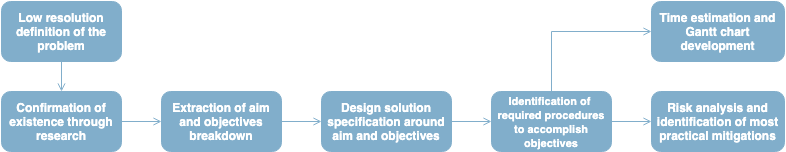
\includegraphics[width=1\textwidth]{initial_analysis.png}
	\caption{Illustration of initial analysis}
	\label{fig:INITIAL_ANALYSIS}
\end{figure}

\section{Development methodology}
The artefact is built inline with the agile software development framework to ensure the development of the artefact is well-structured and to improve time management. Because agile has been designed around production software, it includes a step of releasing the code or code changes once per cycle. As an adaptation to the use case of this artefact, the release step is replaced with an evaluation of test results from previous steps. The difference between the outcome of testing and the aims of the artefact constitutes the feedback.

After development and testing, the code is pushed to the GitHub version control management framework. The reason is to ensure the code can be cloned on multiple testing machines. Moreover, it allows for changes to be tracked and allows for the rollback of issues uncovered in the later development stages.

\begin{figure}[b]
	\centering
	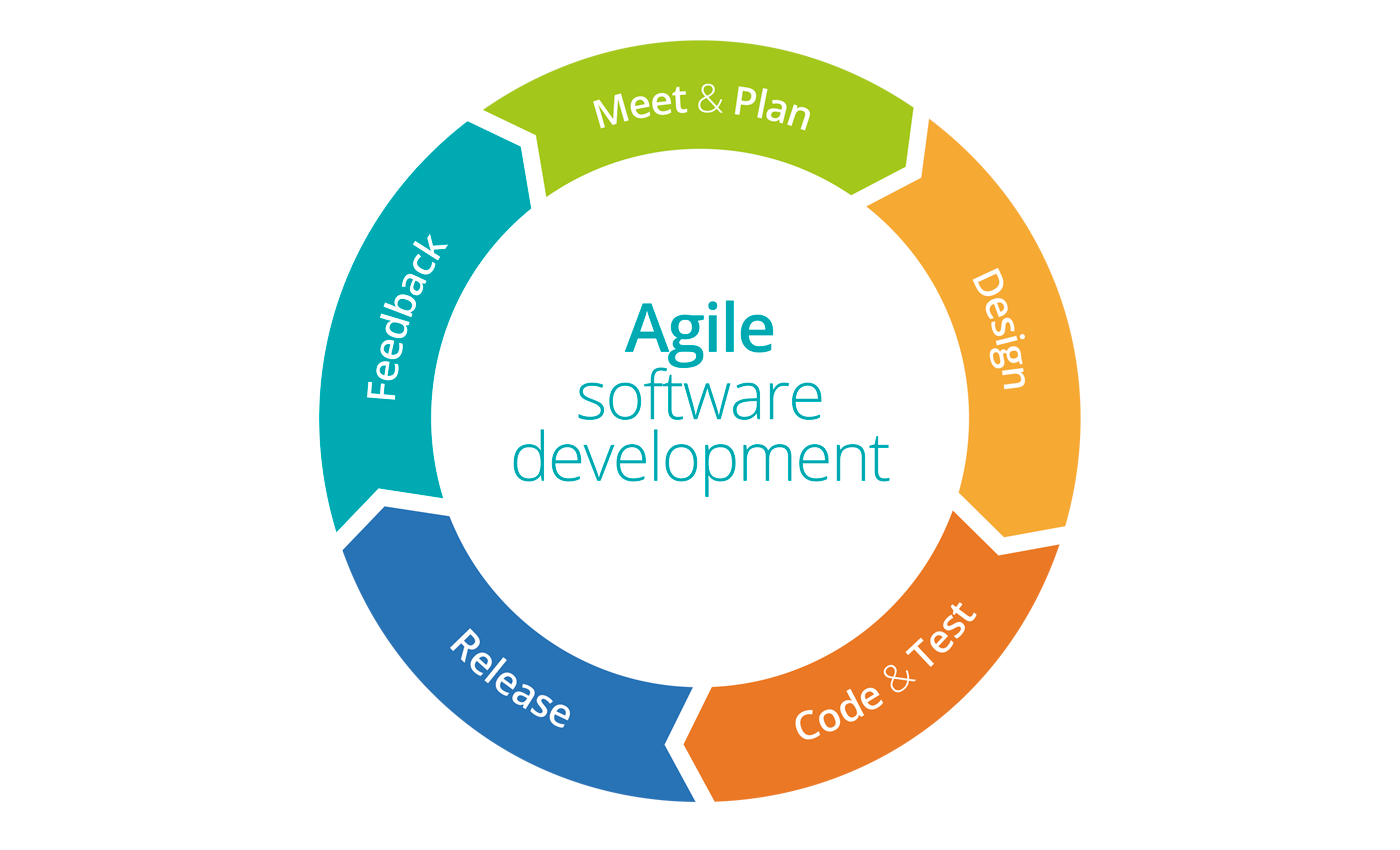
\includegraphics[width=0.42\textwidth]{agile.png}
	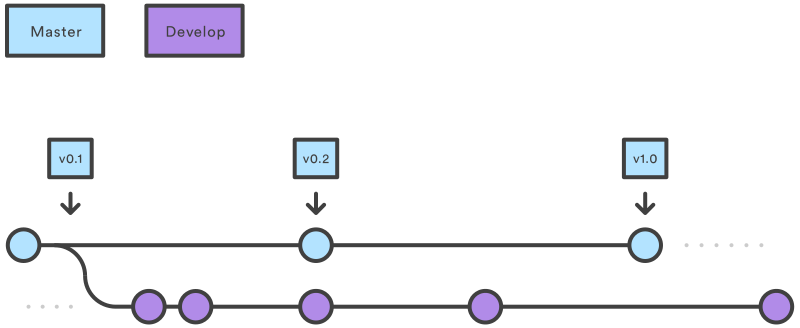
\includegraphics[width=0.57\textwidth]{git.png}
	\caption{Agile development phases (left) and Git flow (right)}
	\label{fig:INITIAL_ANALYSIS}
\end{figure}

\section{Artefact design}
The functional outcome of this dissertation is composed of two pieces of software. The first is the GSB performance assessor used to measure its classification accuracy. This tool will perform an evaluation using both the browser in a realistic scenario and the GSB API. The second is the classifier used to predict whether an URL points to a phishing page or not.

\subsection{GSB performance assessor}
The GSB performance assessor is written in Python 3 and uses the Selenium framework for browser automation. The decision of using Python 3 is justified by its extensive support, readability and ease of use. The selenium framework is chosen because of its well-established reputation in browser automation testing and comprehensive documentation.
The target of the GSB performance assessor is to mimic a user clicking on a phishing link. This scenario captures effectiveness in a real-world setting. The Google Safe Browsing API tester is implemented in Python 3 as well to avoid unnecessary segmentation between the functions of the same software.

\begin{figure}[!b]
	\centering
	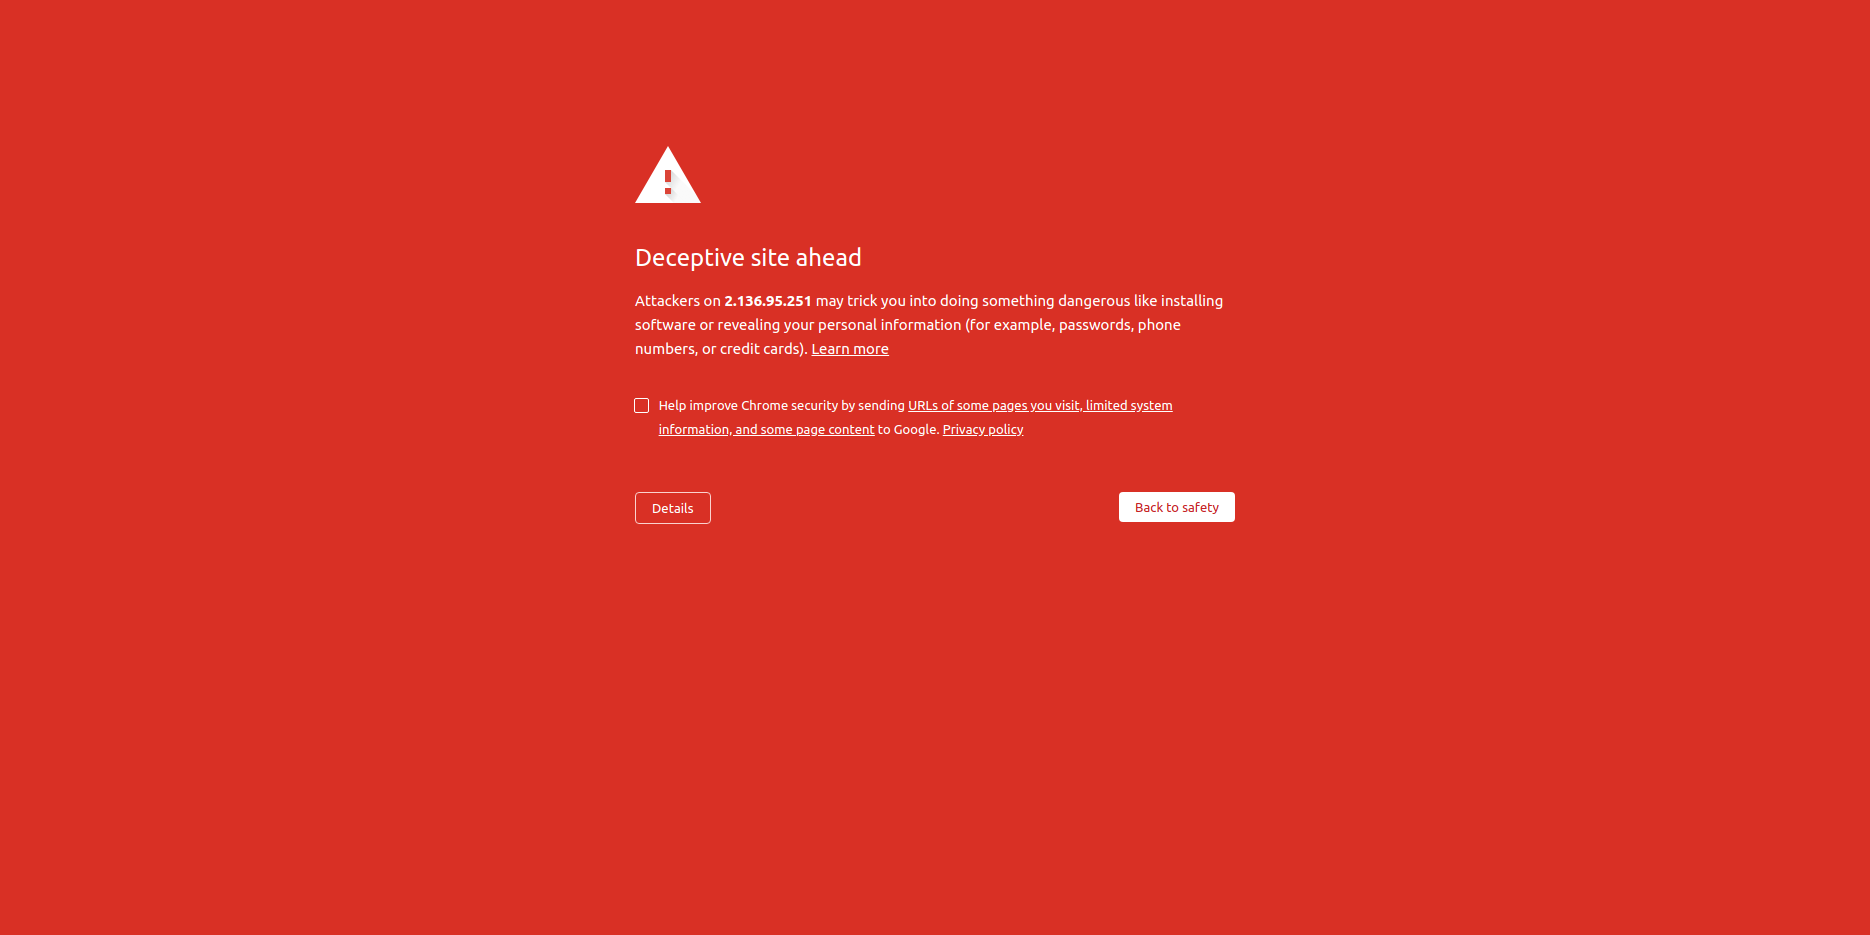
\includegraphics[width=1\textwidth,height=0.29\textheight]{malicious.png}
	\caption{Example of browser's warning page overlay}
	\label{fig:PHISHING_PREVENTED}
\end{figure}

The URLs used in the evaluation process are the latest provided by Phishtank at the moment of testing. These are confirmed to be online and malicious by the PhishTank community. The test executed for each of the malicious URLs starts with loading the default profile of the Google Chrome user. After doing so, the URL is opened, and the page shown by the browser is studied. When a page is classified as malicious, the browser displays a custom page with a warning, as shown in Figure \ref{fig:PHISHING_PREVENTED}. As verification of whether the browser correctly classifies the URL, the tool searches the page's source code for Google's license details. If the browser shows the warning page overlay, the classification is marked as a true-positive. Otherwise, it is recorded as a false-negative.

\subsection{The classifier}
The classifier is the centrepiece of the artefact. It sets to accomplish the dissertation's aim of delivering better protection against phishing than GSB does. The selected approach in designing a competitive anti-phishing detection system is through the identification of key performance indicators that are proven efficient in phishing URL classification. Naturally, the first step in designing the artefact is bringing together information from a wide range of studies on the indices that achieve high classifications accuracy. Following this, the algorithms are trained and compared. The best-performing ones are selected for both hyperparameter tuning and further experimentation with features. UML activity diagram of the classifier illustrated in Figure \ref{fig:UML} and presents the planned flow of actions.

\begin{figure}[!t]
	\centering
	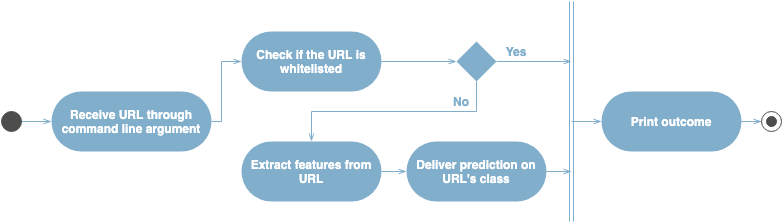
\includegraphics[width=1\textwidth]{uml_horizontal.png}
	\caption{UML acrivity diagram of the classifier}
	\label{fig:UML}
\end{figure}

The machine learning models compared in this dissertation are trained using Python 3 and SciKitLearn \citep{Pedregosa} library. Python is chosen over other programming languages both for the abundance of resources on the subject, and its readability. The actual machine learning algorithms implementations are abstracted by using the SciKit library. Alleviating the complexity of implementing machine learning algorithms saves a significant amount of time. The saved time is allocated toward experimentation and calibration.

The dataset used for feature extraction and training is composed of 100,000 records. It is a compilation made from the first 40,000 benign URLs from \cite{Kumar_Siddharth} and 60,315 phishing URLs from both the same source and PhishTank. The PhishTank URLs used for training are collected with a reasonable time gap between them and the GSB evaluation phase. This way, the model is prevented from having an advantage over GSB.

The set of models used in the experimentation phase is based on the emergent pattern of algorithms used in the Background Study (\ref{chap:background_study}). These are Naive Bayes, Decision Tree, Random Forest and Support Vector Machine. In addition to these, the Multilayered Perceptron is added to test the performance of a neural network.

Model tuning is done using GridSearchCV. GridSearchCV does an exhaustive search over specified parameters and selects the best performing model.

The final wrapper around the whitelist and classifier is implemented using the same programming language. Although better performance can be achieved using a different language, this is done to preserve continuity throughout the artefact.

\section{Evaluation methodology}
The evaluation of GSB's detection mechanism is done in two phases. Firstly the browser will be assessed using newly discovered phishing URLs. After a week of the aforementioned evaluation, the browser will be assessed again using the same data. The rationale behind this lies in the study of how browsers evolve their defences regarding old phishing data.

The evaluation of the machine learning models is based on a set of metrics that cover all the performance areas. In addition, the proposed set makes the process of identifying flaws in calibration easier. The evaluation methodology will coincide with the one presented by some of the studies discussed in the literature review. This is intentional and serves the aim of achieving consistency and offering a fair comparison with the work presented.\newline


\begin{equation}
	\label{eq:precision}
	Precision = \frac{TP}{TP+FP}
\end{equation}
\begin{equation}
	\label{eq:sensitivity}
	Sensitivity = \frac{TP}{TP+FN}
\end{equation}
\begin{equation}
	\label{eq:fmeasure}
	F-Measure = 2*\frac{Precision * Sensitivity}{Precision + Sensitivity}
\end{equation}
\begin{equation}
	\label{eq:accuracy}
	Accuracy = \frac{TP+TN}{TP+TN+FN+FP}
\end{equation}
\newline
\textit{where $TP$ is the number of true positives, $FP$ number of false positives, $TN$ number of true negatives and $FN$ number of false negatives.}

The metrics presented by equations \ref{eq:precision},\ref{eq:sensitivity},\ref{eq:fmeasure} and \ref{eq:accuracy} represent key statistical concepts. A system is said to be precise (\ref{eq:precision}) when it delivers a high level of correct prediction values. Sensitivity \ref{eq:sensitivity}, also known as recall, outlines the system's predisposition in classifying a legitimate URL as being malicious. As the system increases in sensitivity, it reduces the number of false-negatives it produces. For clarification, precision is the ratio between all adequate classification errors and all classification errors. In contrast, recall is the ratio of all classification errors and all existing errors.
The F-Measure (\ref{eq:fmeasure}) is the harmonic mean of precision (the number of correct predictions) and robustness (works well with URLs challenging to classify). It is a composed metric which penalises the extreme values and is meant to provide a single measurement for a system which illustrates the level of optimisation. Finally, the accuracy (\ref{eq:accuracy}) measures the ratio of true-positives and true-negatives.

In addition to these, two other metrics used to provide transparency in model performance are the Receiver Operating Characteristic (ROC) curve and Confusion matrix. The former illustrates how well a model is capable of distinguishing between a phishing URL and a benign one. At the same time, the latter offers a view of the classification performance details of the model.

The final evaluation of the produced classifier is done in comparison to the GSB evaluation results. It is based on the same dataset and metrics to eliminate any variables that may appear between evaluation methods.

\section{Chapter overview}
This chapter presented the methodology used in fulfilling the objectives set objectives in the introduction. It followed the decisions taken the planning, design and development phases and set the evaluation methodology intended to estimate the accomplishment of the aim.